
%%
%% Template chap2.tex
%%

\chapter{Experiment 2: Learning with Thompson Sampling}
\label{cha:expt2}

Let us now turn our attention to active learning. In this chapter,
we investigate the 6 active learning heuristics described in section \ref{sec:heuristics}:
two uncertainty sampling heuristics (entropy and margin), two query
by bagging heuristics (QBB margin and QBB KL), variance minimisation,
and classifier certainty. We then use Thompson sampling to see if
it can automatically filter out the bad heuristics and select the optimal one.


\section{Experimental Protocol}
\label{sec:protocol2}

Out of the four classifiers studied in Chapter \ref{cha:expt1}, only logistic regression
and RBF SVM provide reliable probability estimates. Random forests are able to predict
class probabilities by looking at the distribution of votes. However, we find in practice
that they are not stable (see Appendix for an example). With linear SVMs, the probability 
functionality has not been implemented in scikit-learn. Thus we are left
with only two choices: logistic regression and RBF SVM. The hyperparamters of these classifiers
are the same as those in the previous chapter. 

For the unlabelled pool, we examine two cases. In one case, the pool is balanced, with
an equal number of objects in each class. This allows us to find out the maximum
performance of the heuristics in the best possible scenario. Of course, in real life,
the classes are not evenly distributed. Thus in the second case, we keep the original
class distribution and see if the performance would deteriorate in any way.

Given two choices of classifiers and two ways to construct the
unlabelled pool, we have in total four variations for each dataset and heuristic.
In each run, we do a stratified shuffle split of the training and test data with 10 trials.
All the results including the learning curves are the average of these 10 trials.

All heuristics require probability estimates. Thus we need to start with a partially trained
classifier. Initially, 50 random examples are chosen for training. Then at each step,
we select a random sample of 300 from the unlabelled pool and use the heuristics to rank these candidates. The best
one is then put in our training
set. We keep doing this until a sample size of 300 is achieved. For the committee heuristics,
we use 11 members.

\section{Results and Discussion}
\label{sec:results2}

List of four sets of plots. Colour is kept consistent.

\subsection{Learning with the SDSS Dataset}
\label{sub:learnsdss}

On the next five pages, we plot the results of the experiment on the SDSS dataset.
Figure \ref{fig:sdss_bl_ind} shows the posterior distributions of the
balanced accuracy rate when the training set size reaches 300. The next two pages give us
a more detailed look with learning curves. To avoid cluttering, we plot learning curves
of heuristics that perform worse than random sampling in Figure \ref{fig:sdss_ind_lower}
and those better than random sampling in Figure \ref{fig:sdss_ind_upper}. Finally
Figures \ref{fig:sdss_frequencies}, \ref{fig:sdss_sum_rewards}, and
\ref{fig:sdss_avg_rewards} show the frequency that each heuristic is selected in Thompson
sampling and the dynamics of the rewards over time.

Overall, margin and QBB margin have consistently been the top two heuristics. They can
outperform random sampling by as much as 2\%. The QBB KL heuristic gives a very poor result
in logistic regression, while it is comparable with random sampling with RBF SVMs.
The pool variance heuristic is derived from the Taylor series approximation
of multinomial logistic regression and it seems to work reasonably well with the one-vs-rest
strategy. As we would expect, the theory of SVMs are completely different from that of logistic
regression, making the pool variance heuristic unsuitable here. It is interesting
to see that the pool entropy heuristic also performs quite badly with SVMs, while
the uncertainty sampling entropy approach does very well. The reason for this is unclear.
Finally whether the original data pool is balanced or unbalanced seems to have a very little effect
on the outcome.

Since the bagging technique has been shown to improve the stability of the predictions
\cite{breiman96}, we should expect this method to be no worse the the simple margin approach. The
cost, however, is that it now takes $B$ times longer to calculate the scores, where $B$ is the size
of the committee.

For the Thompson sampling, it seems that even under the very simplifying assumption 
of a normal prior and a normal likelihood, the algorithm still manages to automatically detect
the optimal heuristic. In most cases, the algorithm discovers the margin heuristic to
be optimal after only around 50 samples. Although Thompson sampling doesn't perform as well
as using the margin heuristic alone, this is expected since it needs to do some exploration.
Still, it gives us the third best learning curve in all cases, after margin and QBB magin.
Finally, there is indeed the problem of drifting in the mean of the rewards. It would be
interesting to find out how much quicker the algorithm can recognise the optimal heuristic
if we were to implement the Dynamic Thompson Sampling method.


\begin{figure}[p]
	\centering
	\begin{subfigure}{\textwidth}
		\centering
		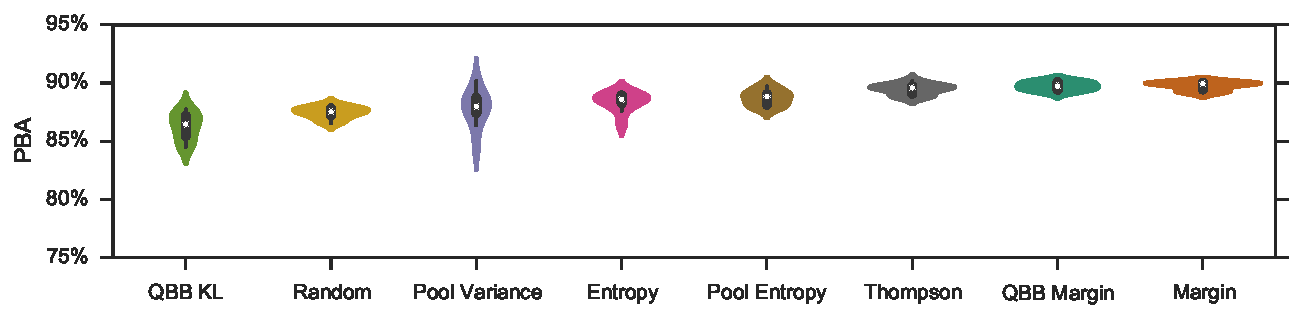
\includegraphics[width=\textwidth]{figures/5_active/sdss_bl_ind_violin}
		\caption{Balanced pool and logistic regression}
		\label{fig:sdss_bl_ind_violin}
	\end{subfigure}
	\begin{subfigure}{\textwidth}
		\centering
		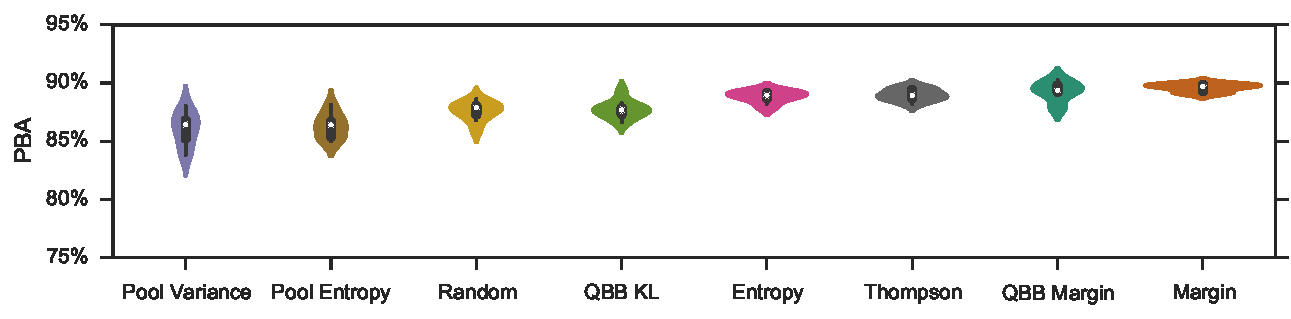
\includegraphics[width=\linewidth]{figures/5_active/sdss_br_ind_violin}
		\caption{Balanced pool and RBF SVM}
		\label{fig:sdss_br_ind_violin}
	\end{subfigure}
	\begin{subfigure}{\textwidth}
		\centering
		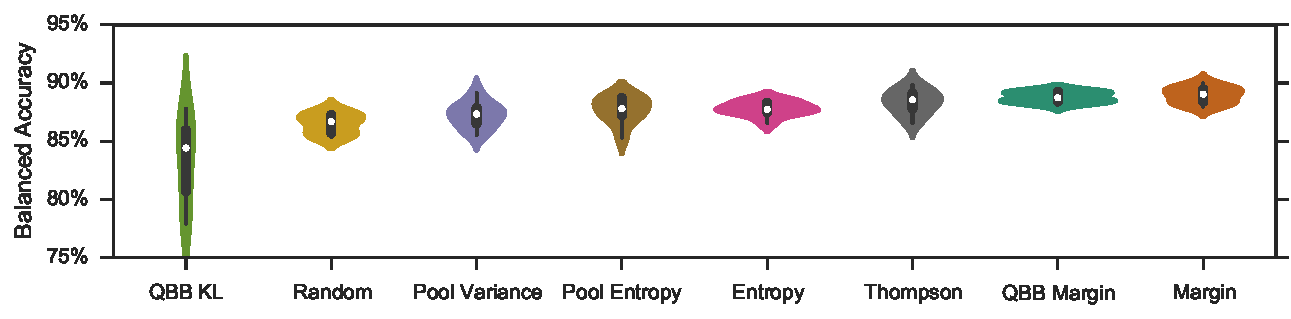
\includegraphics[width=\textwidth]{figures/5_active/sdss_ul_ind_violin}
		\caption{Unbalanced pool and logistic regression}
		\label{fig:sdss_ul_ind_violin}
	\end{subfigure}
	\begin{subfigure}{\textwidth}
		\centering
		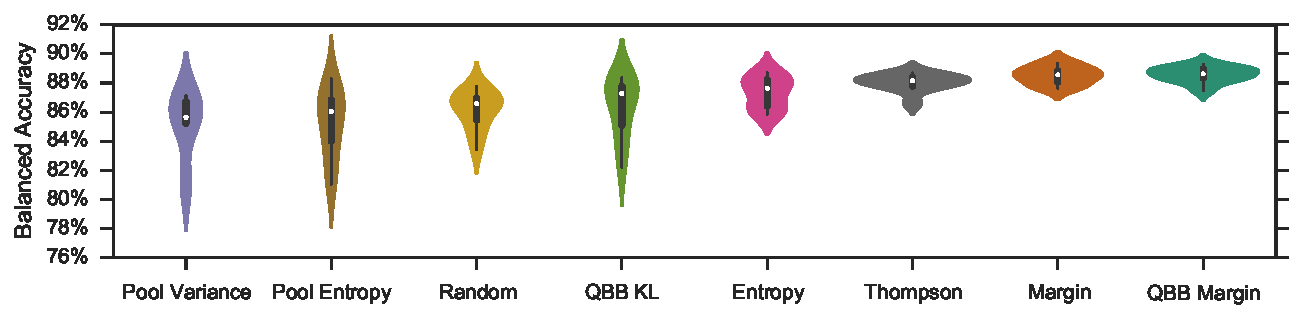
\includegraphics[width=\linewidth]{figures/5_active/sdss_ur_ind_violin}
		\caption{Unbalanced pool and RBF SVM}
		\label{fig:sdss_ur_ind_violin}
	\end{subfigure}
	\caption[Violin plots of balanced accuracy rate (SDSS)]{
		Posterior distributions of the balanced accuracy rate when the SDSS training set size reaches 300: Overall, with the exception of QBB KL and pool variance, all the other
		heuristics manage to outperform random sampling. Both margin and QBB margin are consistently in the top two, with Thompson sampling always at third place. This is expected
		since there is always some exploration in Thompson sampling. Although the pool
		variance heuristic on average outperforms random sampling slightly, it has quite a
		bit of variable and thus unreliable.}
	\label{fig:sdss_bl_ind}
\end{figure}


\begin{figure}[p]
	\centering
	\begin{subfigure}{.5\textwidth}
		\centering
		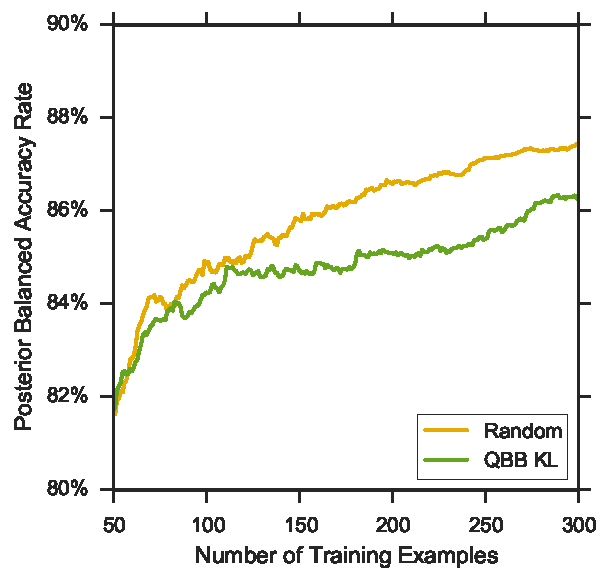
\includegraphics[width=\textwidth]{figures/5_active/sdss_bl_ind_lower}
		\caption{Balanced pool and logistic regression}
		\label{fig:sdss_bl_ind_lower}
	\end{subfigure}%
	\begin{subfigure}{.5\textwidth}
		\centering
		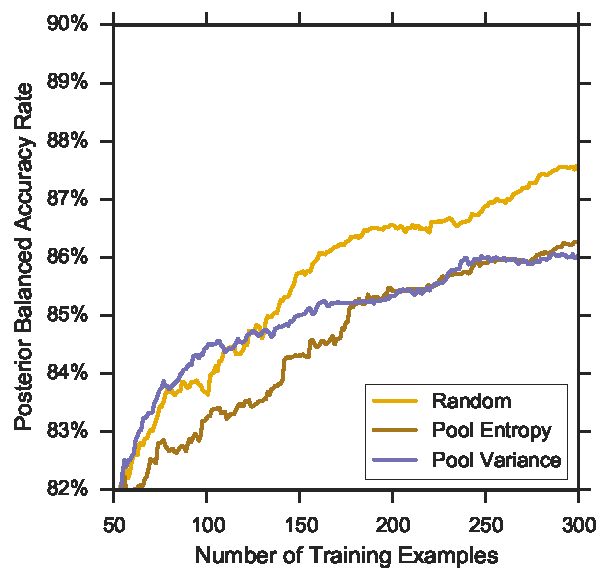
\includegraphics[width=\linewidth]{figures/5_active/sdss_br_ind_lower}
		\caption{Balanced pool and RBF SVM}
		\label{fig:sdss_br_ind_lower}
	\end{subfigure}
	\begin{subfigure}{.5\textwidth}
		\centering
		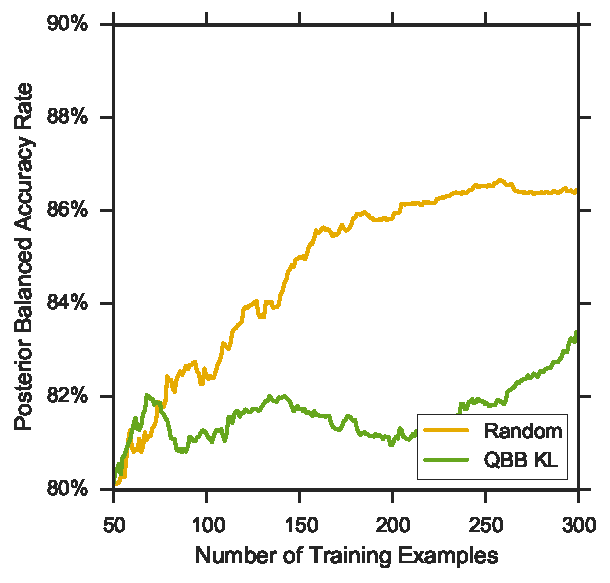
\includegraphics[width=\textwidth]{figures/5_active/sdss_ul_ind_lower}
		\caption{Unbalanced pool and logistic regression}
		\label{fig:sdss_ul_ind_lower}
	\end{subfigure}%
	\begin{subfigure}{.5\textwidth}
		\centering
		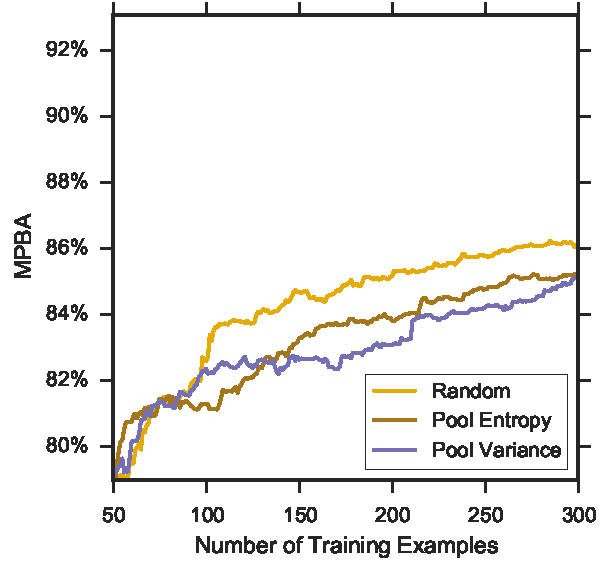
\includegraphics[width=\linewidth]{figures/5_active/sdss_ur_ind_lower}
		\caption{Unbalanced pool and RBF SVM}
		\label{fig:sdss_ur_ind_lower}
	\end{subfigure}
	\caption[Learning curves of heuristics worse than random (SDSS)]{
		Learning curves (average of 10 trials) of heuristics that perform worse than random sampling in the SDSS dataset: We can clearly see that with logistic regression,
		QBB KL performs much worse than random sampling. For 
		RBF SVM, the bad heuristics are pool variance and pool entropy. The underperformance
		of the pool variance heuristic is expected since the theory does not quite apply
		to SVMs.}
	\label{fig:sdss_ind_lower}
\end{figure}


\begin{figure}[p]
	\centering
	\begin{subfigure}{.5\textwidth}
		\centering
		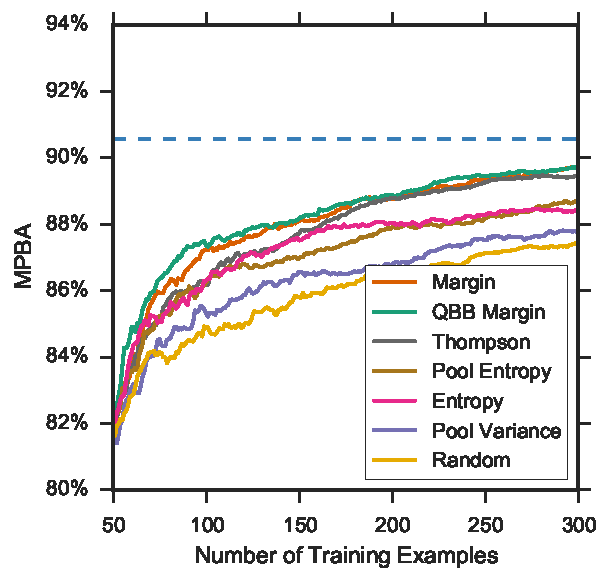
\includegraphics[width=\textwidth]{figures/5_active/sdss_bl_ind_upper}
		\caption{Balanced pool and logistic regression}
		\label{fig:sdss_bl_ind_upper}
	\end{subfigure}%
	\begin{subfigure}{.5\textwidth}
		\centering
		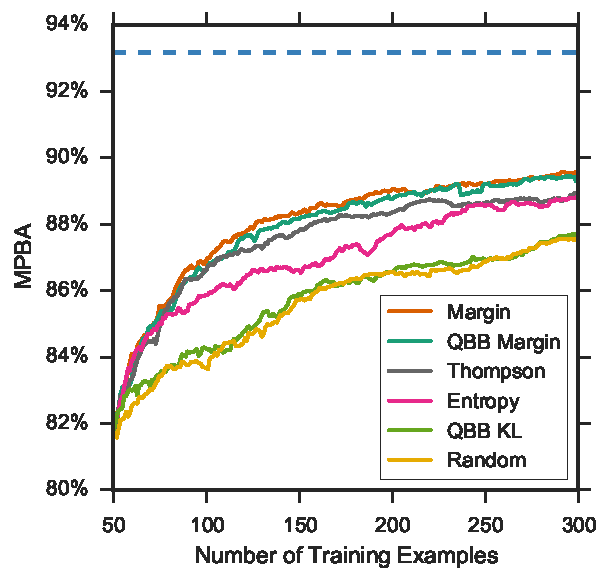
\includegraphics[width=\linewidth]{figures/5_active/sdss_br_ind_upper}
		\caption{Balanced pool and RBF SVM}
		\label{fig:sdss_br_ind_upper}
	\end{subfigure}
	\begin{subfigure}{.5\textwidth}
		\centering
		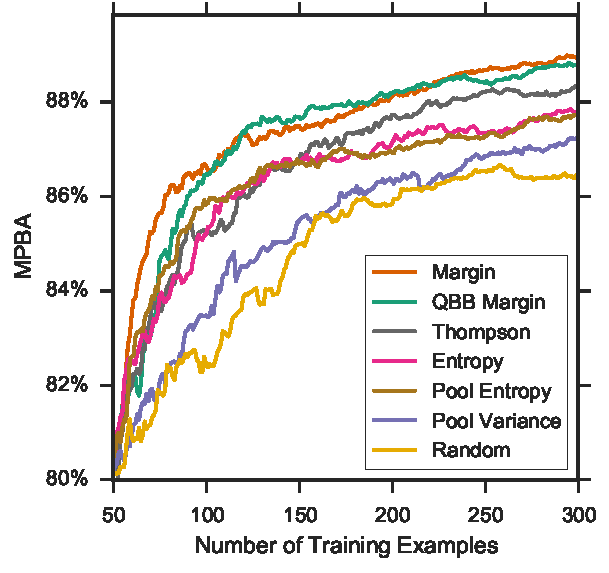
\includegraphics[width=\textwidth]{figures/5_active/sdss_ul_ind_upper}
		\caption{Unbalanced pool and logistic regression}
		\label{fig:sdss_ul_ind_upper}
	\end{subfigure}%
	\begin{subfigure}{.5\textwidth}
		\centering
		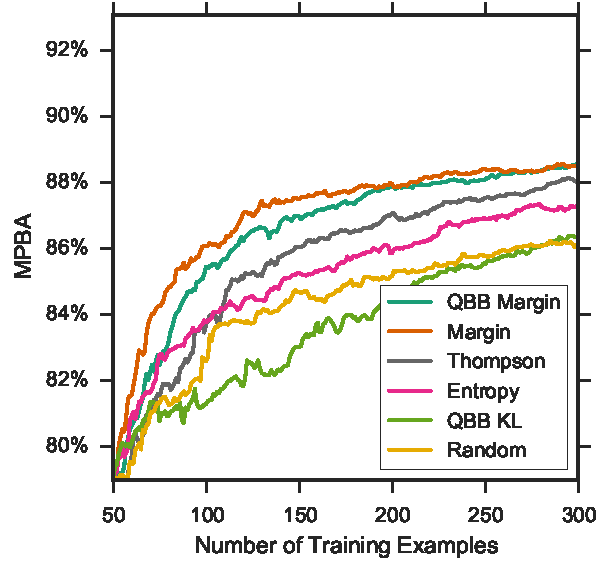
\includegraphics[width=\linewidth]{figures/5_active/sdss_ur_ind_upper}
		\caption{Unbalanced pool and RBF SVM}
		\label{fig:sdss_ur_ind_upper}
	\end{subfigure}
	\caption[Learning curves of heuristics better than random (SDSS)]{
		Learning curves (average of 10 trials) of heuristics that outperform random sampling in the SDSS dataset.}
	\label{fig:sdss_ind_upper}
\end{figure}


\begin{figure}[p]
	\centering
	\begin{subfigure}{.5\textwidth}
		\centering
		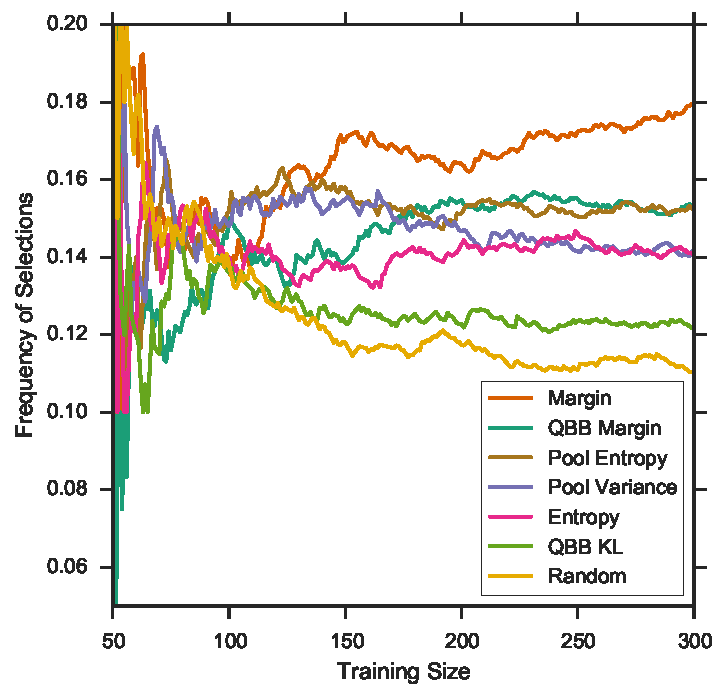
\includegraphics[width=\textwidth]{figures/5_thompson/sdss_bl_frequencies}
		\caption{Balanced pool and logistic regression}
		\label{fig:sdss_bl_frequencies}
	\end{subfigure}%
	\begin{subfigure}{.5\textwidth}
		\centering
		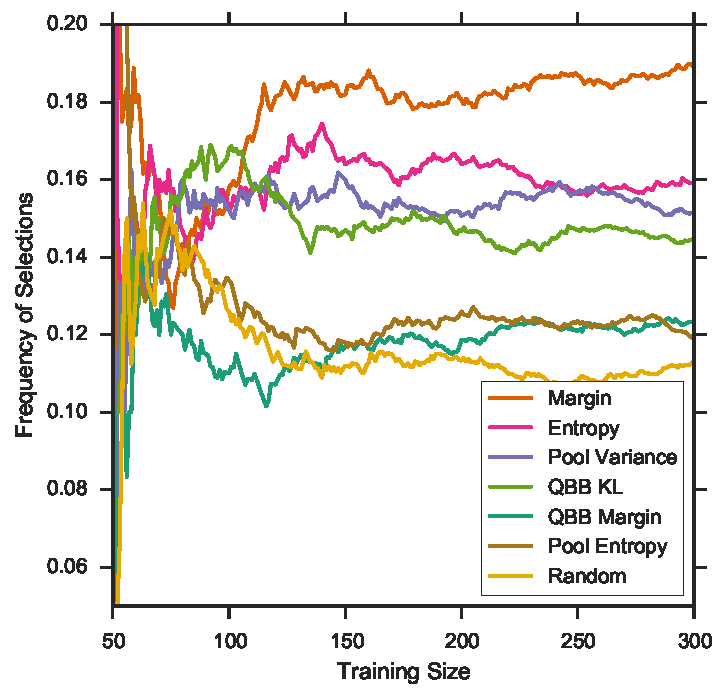
\includegraphics[width=\linewidth]{figures/5_thompson/sdss_br_frequencies}
		\caption{Balanced pool and RBF SVM}
		\label{fig:sdss_br_frequencies}
	\end{subfigure}
	\begin{subfigure}{.5\textwidth}
		\centering
		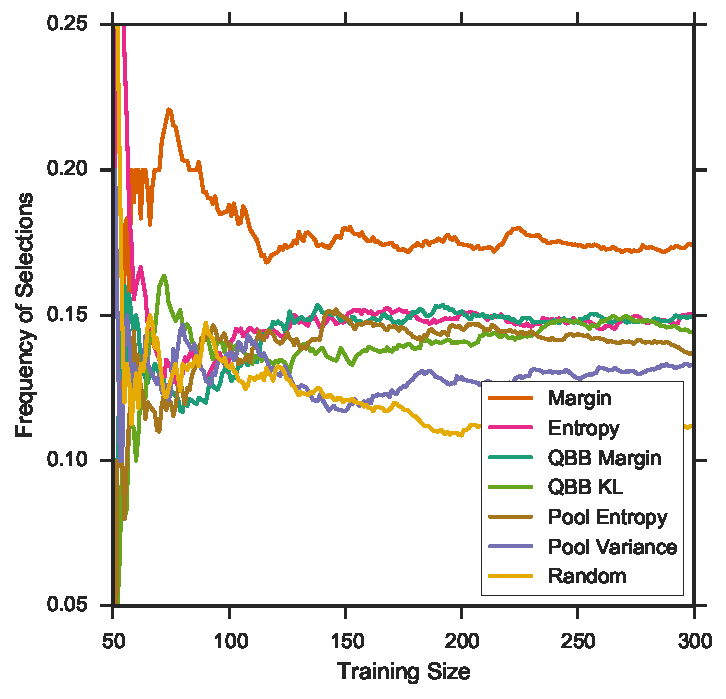
\includegraphics[width=\textwidth]{figures/5_thompson/sdss_ul_frequencies}
		\caption{Unbalanced pool and logistic regression}
		\label{fig:sdss_ul_frequencies}
	\end{subfigure}%
	\begin{subfigure}{.5\textwidth}
		\centering
		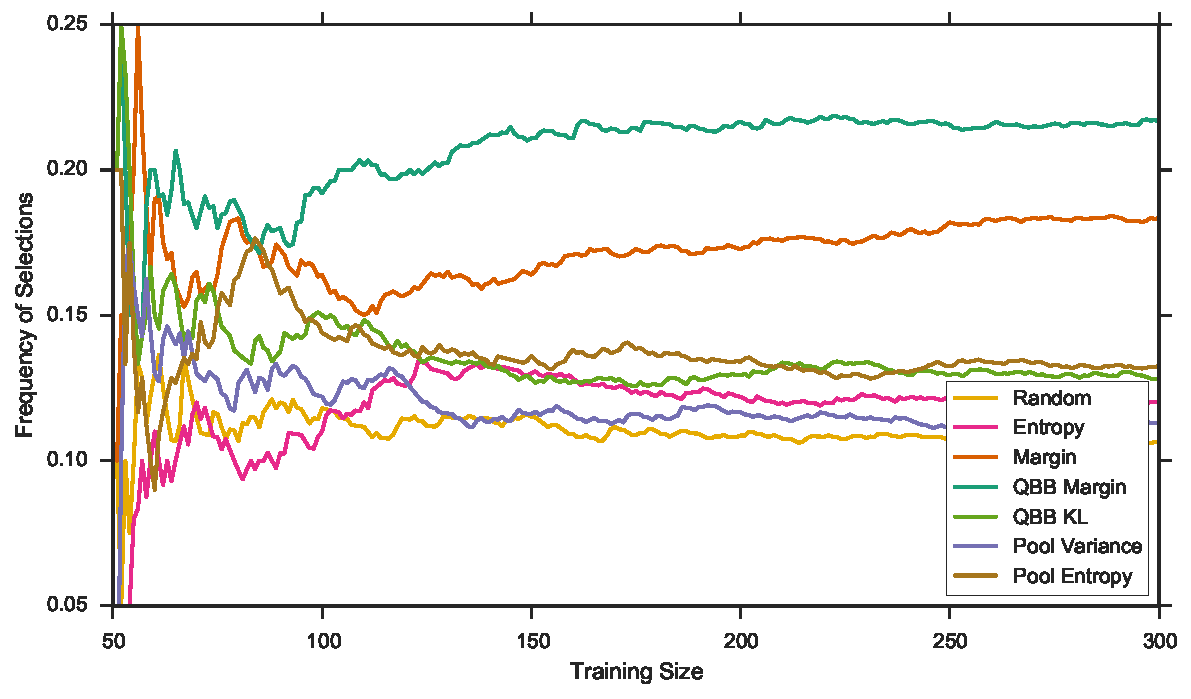
\includegraphics[width=\linewidth]{figures/5_thompson/sdss_ur_frequencies}
		\caption{Unbalanced pool and RBF SVM}
		\label{fig:sdss_ur_frequencies}
	\end{subfigure}
	\caption[Heuristic selection frequency (SDSS)]{
		Heuristic selection frequency in Thopmson sampling with the SDSS dataset.}
	\label{fig:sdss_frequencies}
\end{figure}


\begin{figure}[p]
	\centering
	\begin{subfigure}{.5\textwidth}
		\centering
		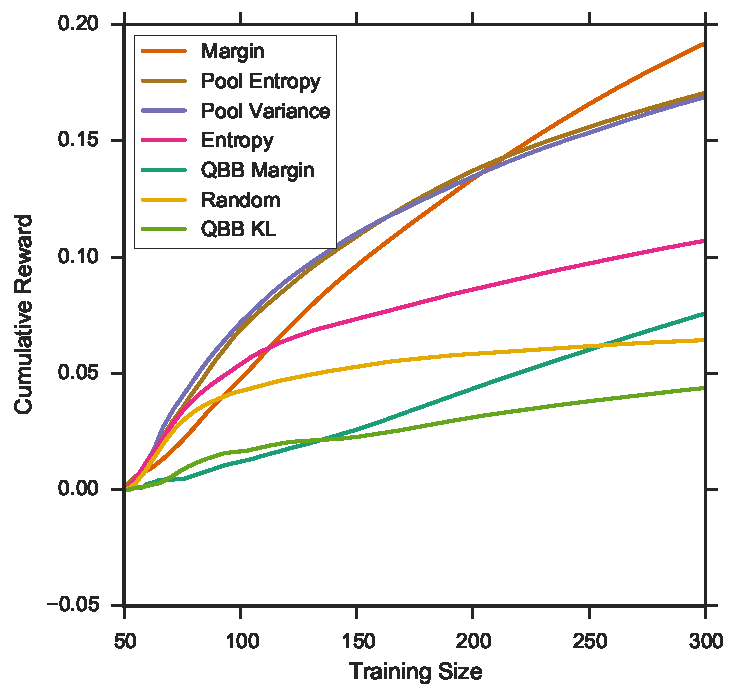
\includegraphics[width=\textwidth]{figures/5_thompson/sdss_bl_sum_rewards}
		\caption{Balanced pool and logistic regression}
		\label{fig:sdss_bl_sum_rewards}
	\end{subfigure}%
	\begin{subfigure}{.5\textwidth}
		\centering
		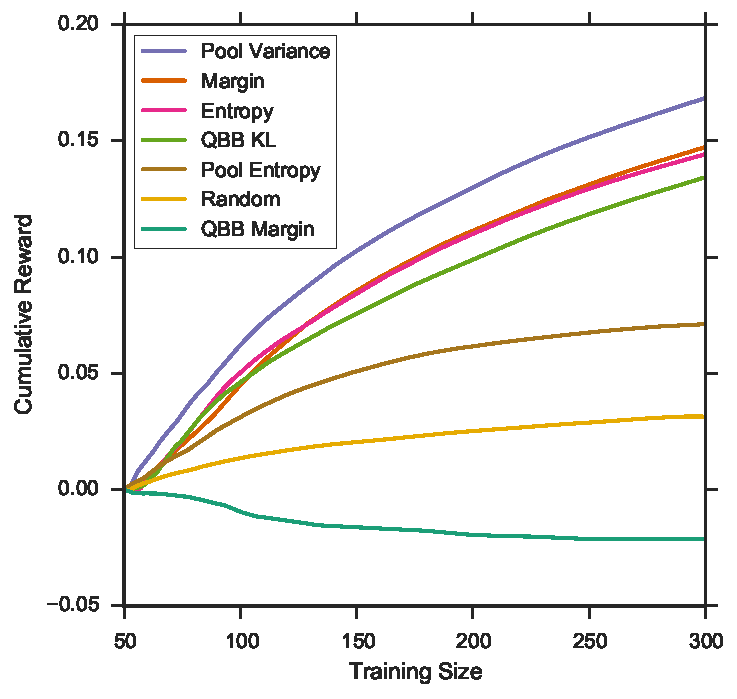
\includegraphics[width=\linewidth]{figures/5_thompson/sdss_br_sum_rewards}
		\caption{Balanced pool and RBF SVM}
		\label{fig:sdss_br_sum_rewards}
	\end{subfigure}
	\begin{subfigure}{.5\textwidth}
		\centering
		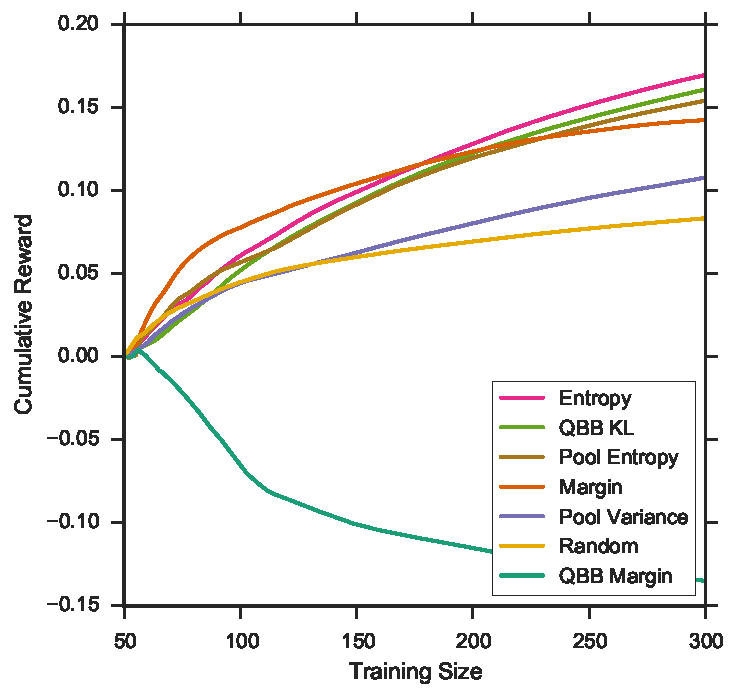
\includegraphics[width=\textwidth]{figures/5_thompson/sdss_ul_sum_rewards}
		\caption{Unbalanced pool and logistic regression}
		\label{fig:sdss_ul_sum_rewards}
	\end{subfigure}%
	\begin{subfigure}{.5\textwidth}
		\centering
		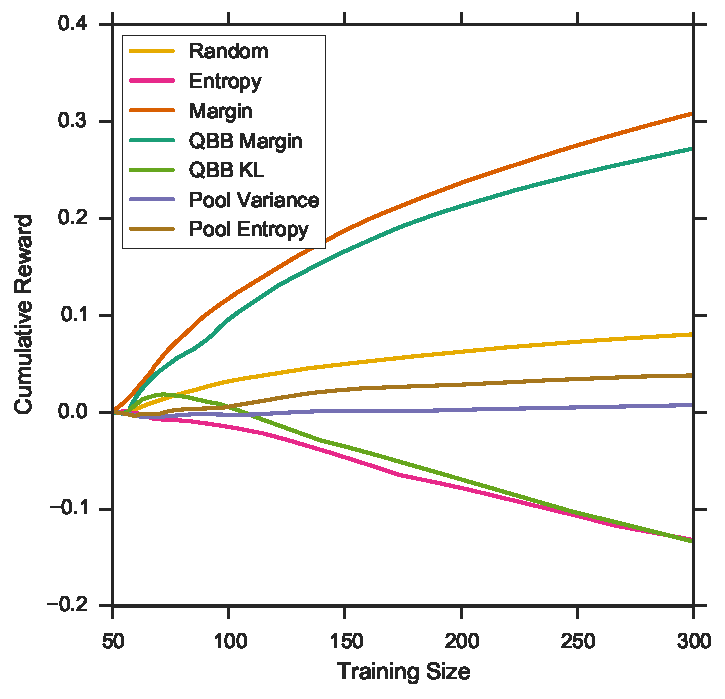
\includegraphics[width=\linewidth]{figures/5_thompson/sdss_ur_sum_rewards}
		\caption{Unbalanced pool and RBF SVM}
		\label{fig:sdss_ur_sum_rewards}
	\end{subfigure}
	\caption[Cumulative reward of heuristics (SDSS)]{
		Cumulative reward in Thompson sampling with the SDSS dataset.}
	\label{fig:sdss_sum_rewards}
\end{figure}


\begin{figure}[p]
	\centering
	\begin{subfigure}{.5\textwidth}
		\centering
		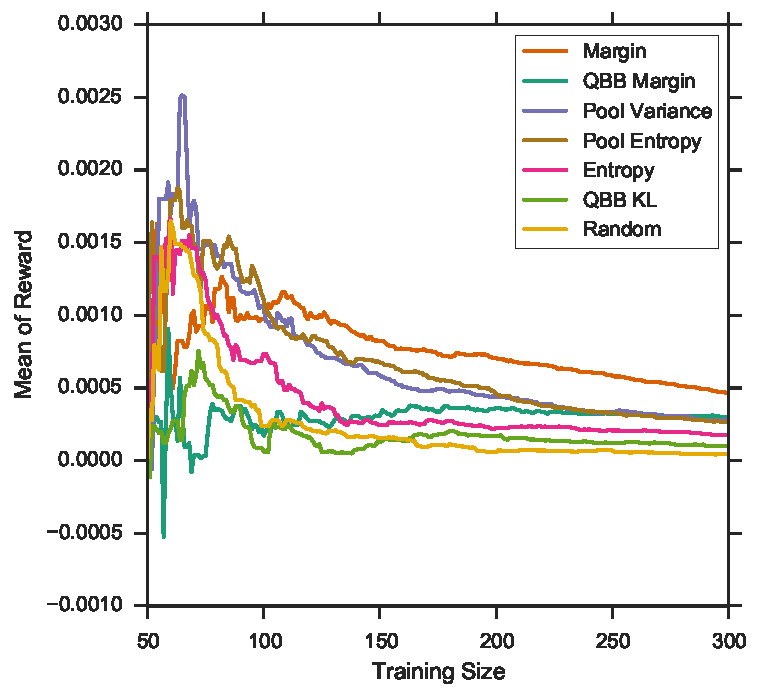
\includegraphics[width=\textwidth]{figures/5_thompson/sdss_bl_avg_rewards}
		\caption{Balanced pool and logistic regression}
		\label{fig:sdss_bl_avg_rewards}
	\end{subfigure}%
	\begin{subfigure}{.5\textwidth}
		\centering
		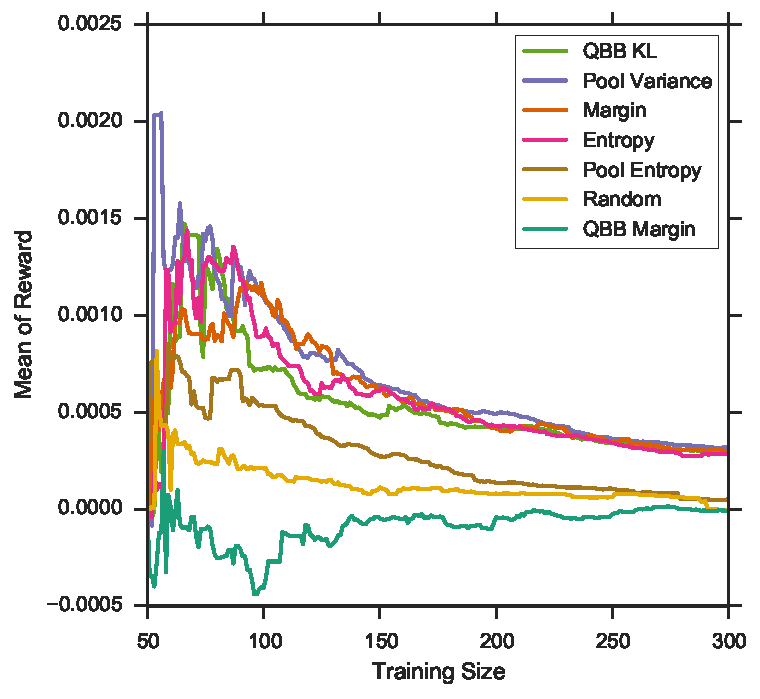
\includegraphics[width=\linewidth]{figures/5_thompson/sdss_br_avg_rewards}
		\caption{Balanced pool and RBF SVM}
		\label{fig:sdss_br_avg_rewards}
	\end{subfigure}
	\begin{subfigure}{.5\textwidth}
		\centering
		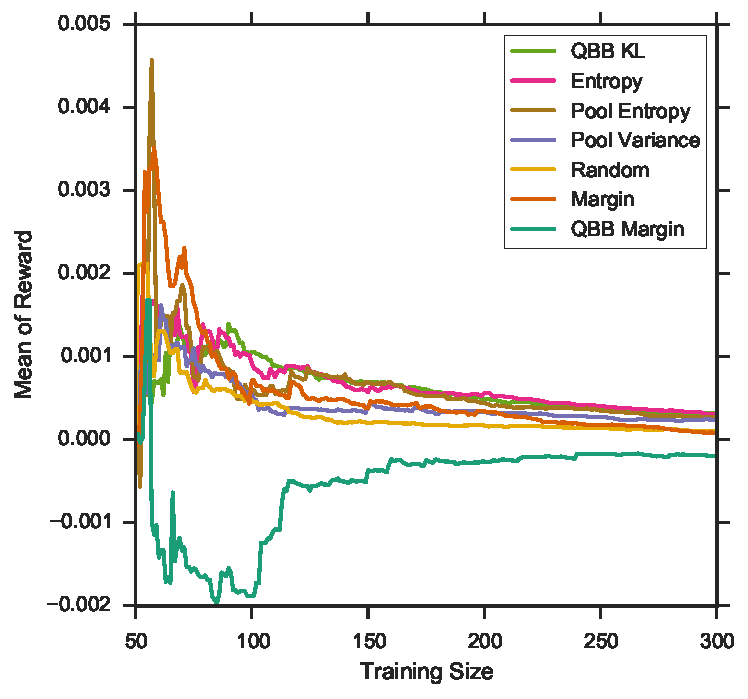
\includegraphics[width=\textwidth]{figures/5_thompson/sdss_ul_avg_rewards}
		\caption{Unbalanced pool and logistic regression}
		\label{fig:sdss_ul_avg_rewards}
	\end{subfigure}%
	\begin{subfigure}{.5\textwidth}
		\centering
		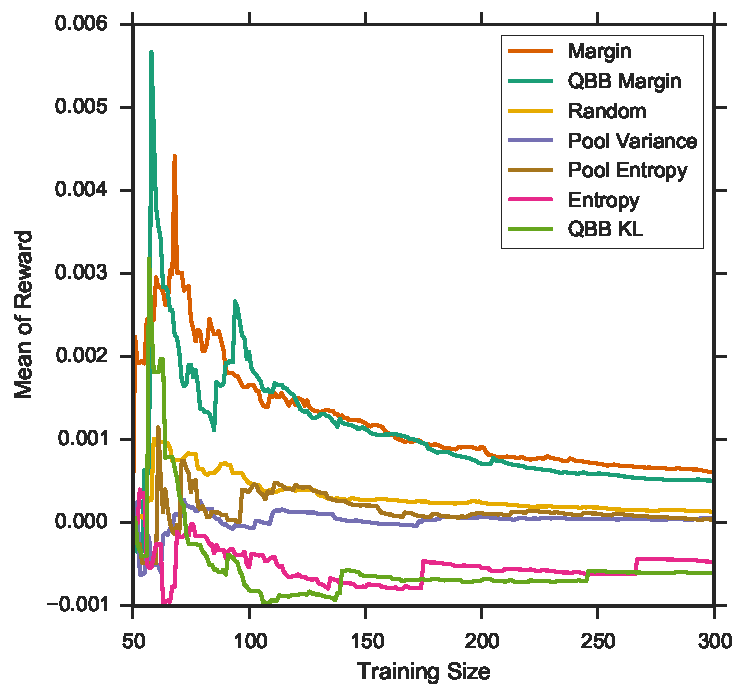
\includegraphics[width=\linewidth]{figures/5_thompson/sdss_ur_avg_rewards}
		\caption{Unbalanced pool and RBF SVM}
		\label{fig:sdss_ur_avg_rewards}
	\end{subfigure}
	\caption[Mean reward of heuristics (SDSS)]{
		Mean reward in Thompson sampling with the SDSS dataset.}
	\label{fig:sdss_avg_rewards}
\end{figure}


% % % % % % % % % % % % % % % % % % % % % % % % % % % % % % % % % % % % % % % % % % % % % % % % % %
\subsection{Learning with the VST ATLAS Dataset}
\label{sub:learnvstatlas}

Figures \ref{fig:vstatlas_bl_ind} to \ref{fig:vstatlas_avg_rewards} show the results of the experiment on the VST ATLAS dataset.
The organisation of the plots is the same as the SDSS.
The VST ATLAS has a much cleaner dataset, and the active learning seems to work
much better here. Margin, QBB margin, and entropy all perform much better than random sampling.
At times, especially when the dataset is unbalanced, the difference in performance can
be as great as 9\%. When using logistic regression, everything performs better
than random, including the QBB KL heuristic.

\begin{figure}[p]
	\centering
	\begin{subfigure}{\textwidth}
		\centering
		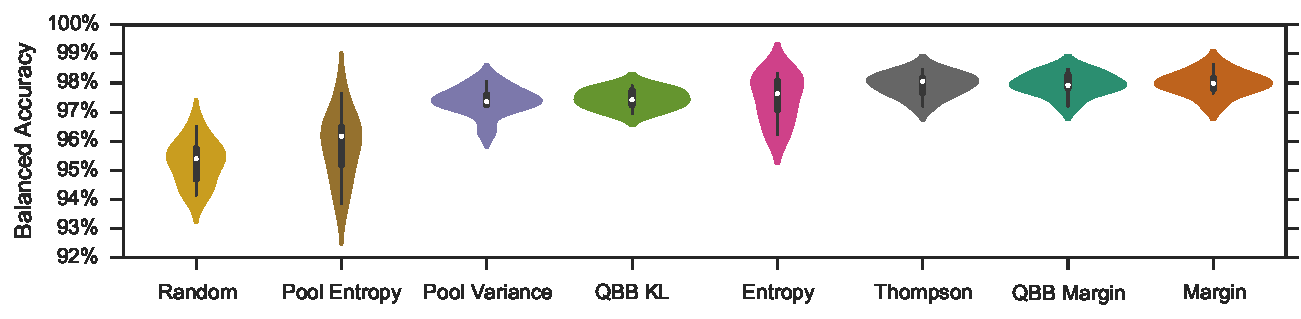
\includegraphics[width=\textwidth]{figures/5_active/vstatlas_bl_ind_violin}
		\caption{Balanced unlabelled pool and logistic regression}
		\label{fig:vstatlas_bl_ind_violin}
	\end{subfigure}\\
	\begin{subfigure}{\textwidth}
		\centering
		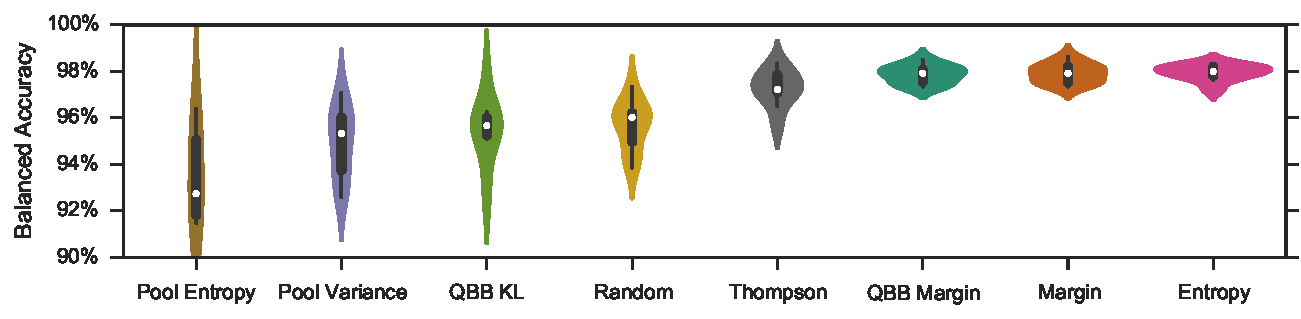
\includegraphics[width=\linewidth]{figures/5_active/vstatlas_br_ind_violin}
		\caption{Balanced unlabelled pool and RBF SVM}
		\label{fig:vstatlas_br_ind_violin}
	\end{subfigure}\\
	\begin{subfigure}{\textwidth}
		\centering
		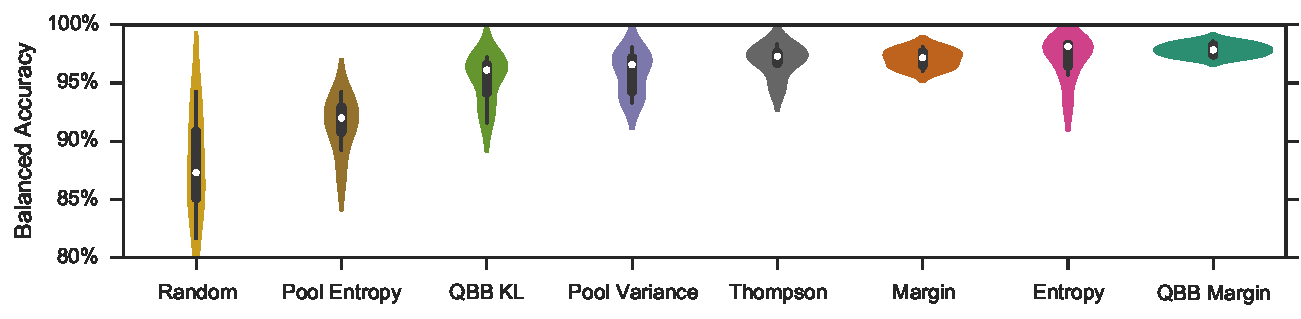
\includegraphics[width=\textwidth]{figures/5_active/vstatlas_ul_ind_violin}
		\caption{Unbalanced unlabelled pool and logistic regression}
		\label{fig:vstatlas_ul_ind_violin}
	\end{subfigure}\\
	\begin{subfigure}{\textwidth}
		\centering
		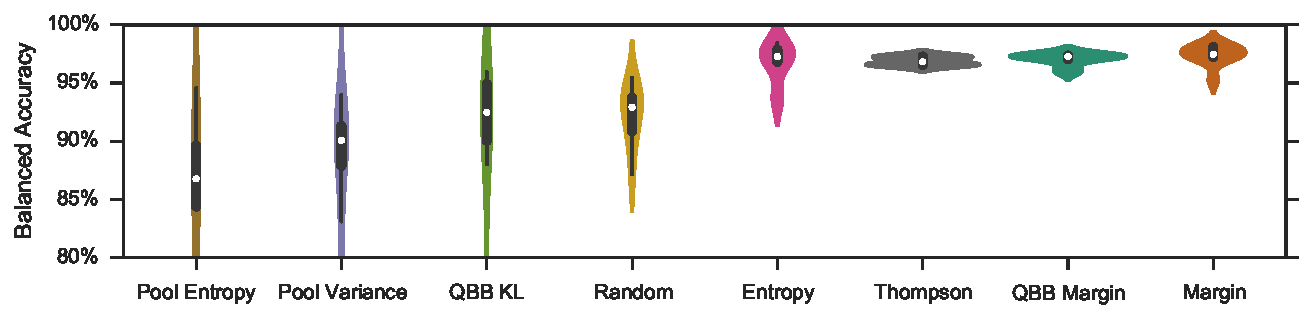
\includegraphics[width=\linewidth]{figures/5_active/vstatlas_ur_ind_violin}
		\caption{Unbalanced unlabelled pool and RBF SVM}
		\label{fig:vstatlas_ur_ind_violin}
	\end{subfigure}
	\caption[Violin plots of balanced accuracy rate (VST ATLAS)]{
		Posterior distributions of the balanced accuracy rate when the VST ATLAS training set size reaches 300: Overall, all heuristics outperform random sampling when we use logistic regression. With RBF SVM, the two pool heuristics and QBB KL don't seem to do as well.
		In particular, as we can see in Figure \ref{fig:vstatlas_ur_ind_violin}, when the classes are unbalanced, these three heuristics become very unreliable.}
	\label{fig:vstatlas_bl_ind}
\end{figure}


\begin{figure}[p]
	\centering
	\begin{subfigure}{.5\textwidth}
		\centering
		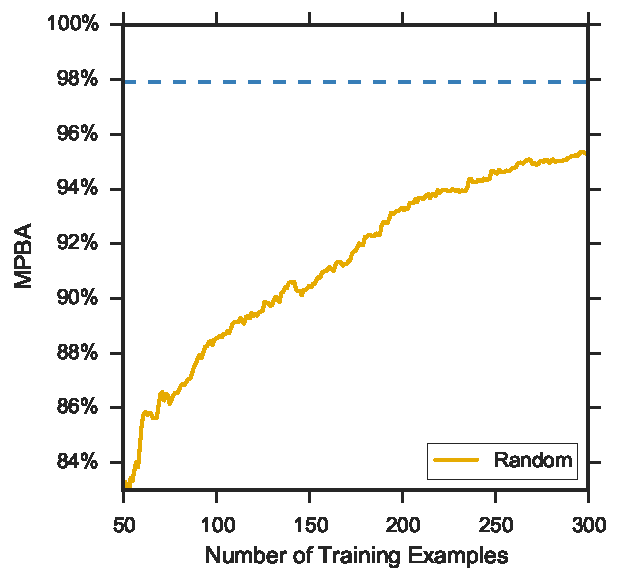
\includegraphics[width=\textwidth]{figures/5_active/vstatlas_bl_ind_lower}
		\caption{Balanced pool and logistic regression}
		\label{fig:vstatlas_bl_ind_lower}
	\end{subfigure}%
	\begin{subfigure}{.5\textwidth}
		\centering
		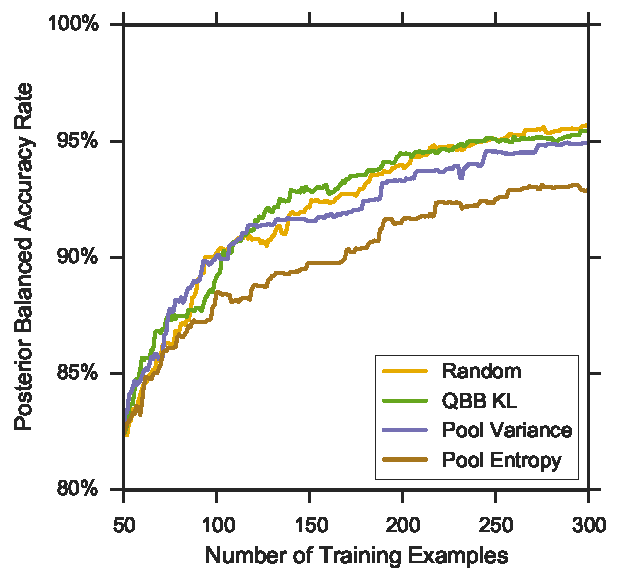
\includegraphics[width=\linewidth]{figures/5_active/vstatlas_br_ind_lower}
		\caption{Balanced pool and RBF SVM}
		\label{fig:vstatlas_br_ind_lower}
	\end{subfigure}
	\begin{subfigure}{.5\textwidth}
		\centering
		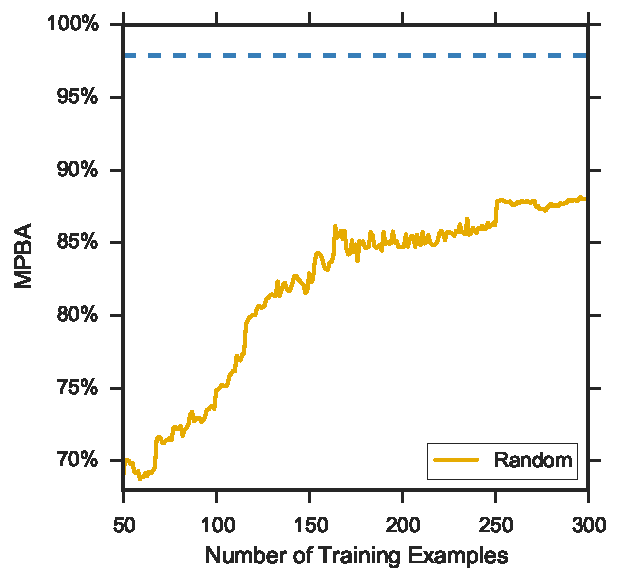
\includegraphics[width=\textwidth]{figures/5_active/vstatlas_ul_ind_lower}
		\caption{Unbalanced pool and logistic regression}
		\label{fig:vstatlas_ul_ind_lower}
	\end{subfigure}%
	\begin{subfigure}{.5\textwidth}
		\centering
		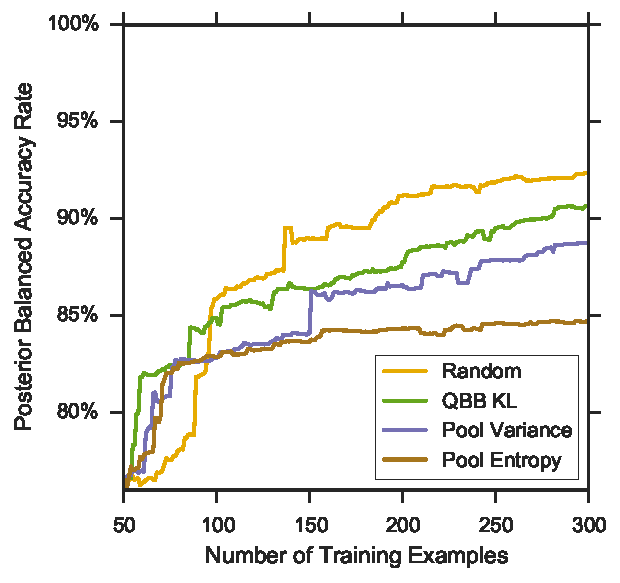
\includegraphics[width=\linewidth]{figures/5_active/vstatlas_ur_ind_lower}
		\caption{Unbalanced pool and RBF SVM}
		\label{fig:vstatlas_ur_ind_lower}
	\end{subfigure}
	\caption[Learning curves of heuristics worse than random (VST ATLAS)]{
		Learning curves (average of 10 trials) of heuristics that perform worse than random sampling in the VST ATLAS dataset: The plots for logistic regression are quite uninteresting
		since all heuristics beat random sampling. In Figure \ref{fig:vstatlas_ur_ind_lower},
		the learning curve for the pool entropy heuristic appears to flatten out after 100 samples.
		}
	\label{fig:vstatlas_ind_lower}
\end{figure}


\begin{figure}[p]
	\centering
	\begin{subfigure}{.5\textwidth}
		\centering
		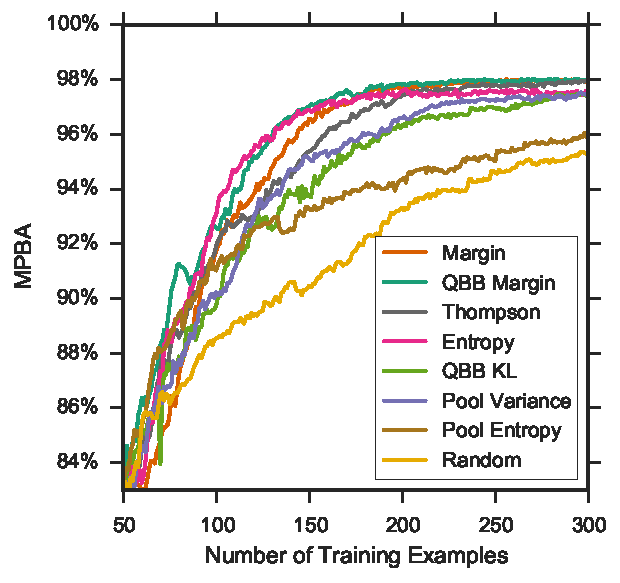
\includegraphics[width=\textwidth]{figures/5_active/vstatlas_bl_ind_upper}
		\caption{Balanced pool and logistic regression}
		\label{fig:vstatlas_bl_ind_upper}
	\end{subfigure}%
	\begin{subfigure}{.5\textwidth}
		\centering
		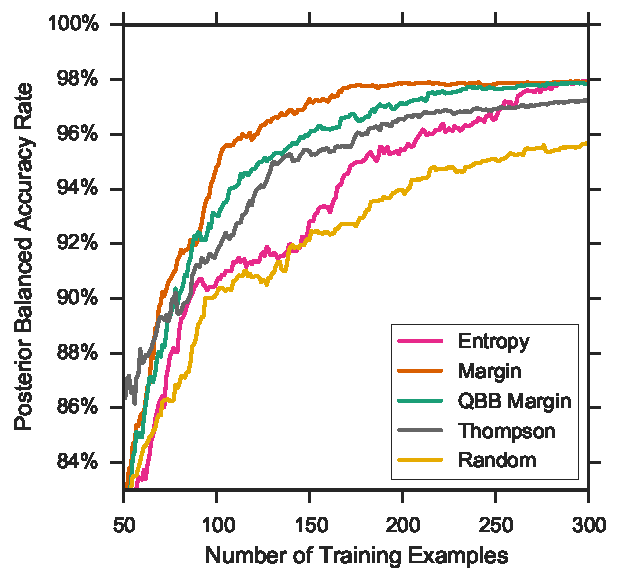
\includegraphics[width=\linewidth]{figures/5_active/vstatlas_br_ind_upper}
		\caption{Balanced pool and RBF SVM}
		\label{fig:vstatlas_br_ind_upper}
	\end{subfigure}
	\begin{subfigure}{.5\textwidth}
		\centering
		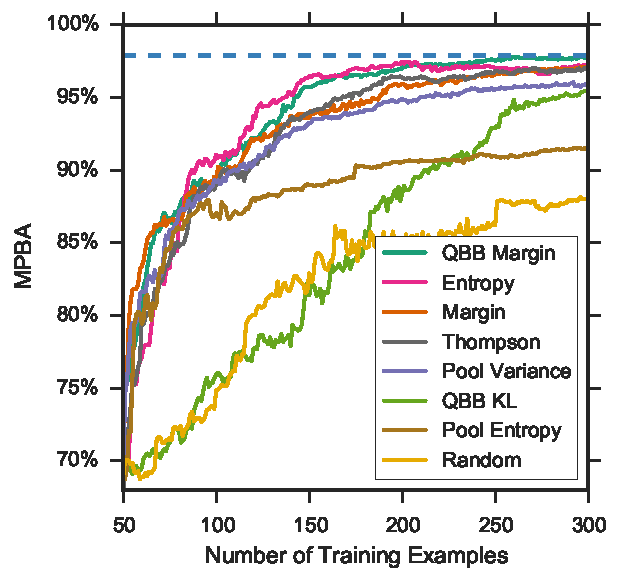
\includegraphics[width=\textwidth]{figures/5_active/vstatlas_ul_ind_upper}
		\caption{Unbalanced pool and logistic regression}
		\label{fig:vstatlas_ul_ind_upper}
	\end{subfigure}%
	\begin{subfigure}{.5\textwidth}
		\centering
		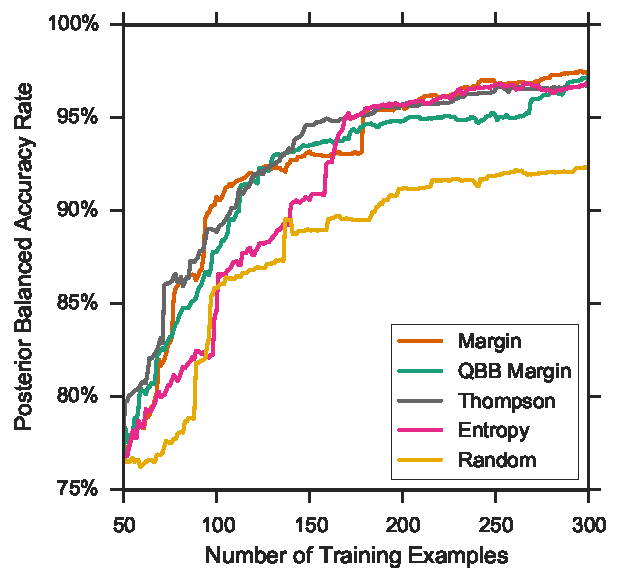
\includegraphics[width=\linewidth]{figures/5_active/vstatlas_ur_ind_upper}
		\caption{Unbalanced pool and RBF SVM}
		\label{fig:vstatlas_ur_ind_upper}
	\end{subfigure}
	\caption[Learning curves of heuristics better than random (VST ATLAS)]{
		Learning curves (average of 10 trials) of heuristics that outperform random sampling in the VST ATLAS dataset.
	}
	\label{fig:vstatlas_ind_upper}
\end{figure}


\begin{figure}[p]
	\centering
	\begin{subfigure}{.5\textwidth}
		\centering
		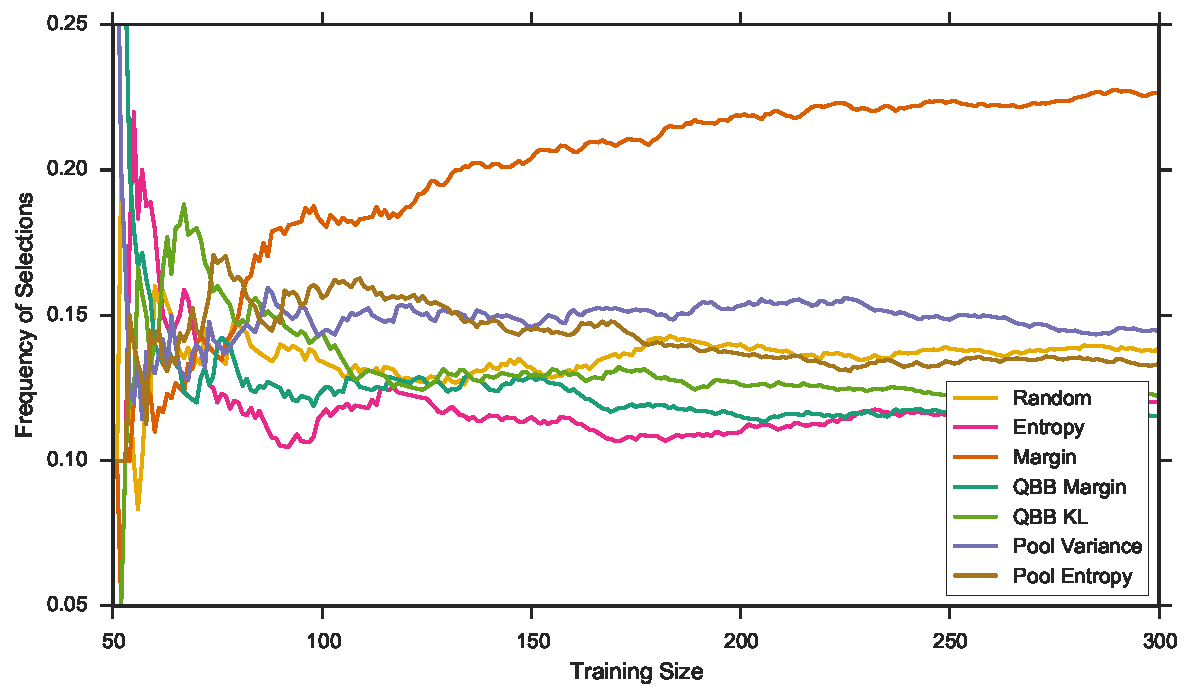
\includegraphics[width=\textwidth]{figures/5_thompson/vstatlas_bl_frequencies}
		\caption{Balanced pool and logistic regression}
		\label{fig:vstatlas_bl_frequencies}
	\end{subfigure}%
	\begin{subfigure}{.5\textwidth}
		\centering
		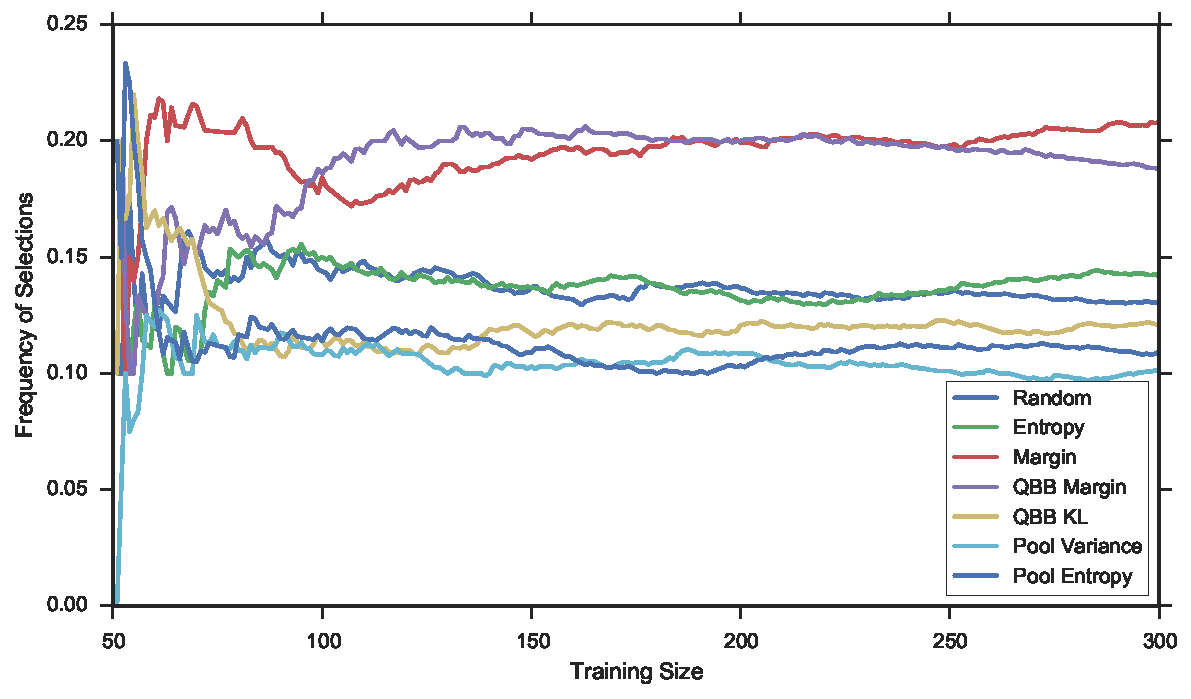
\includegraphics[width=\linewidth]{figures/5_thompson/vstatlas_br_frequencies}
		\caption{Balanced pool and RBF SVM}
		\label{fig:vstatlas_br_frequencies}
	\end{subfigure}
	\begin{subfigure}{.5\textwidth}
		\centering
		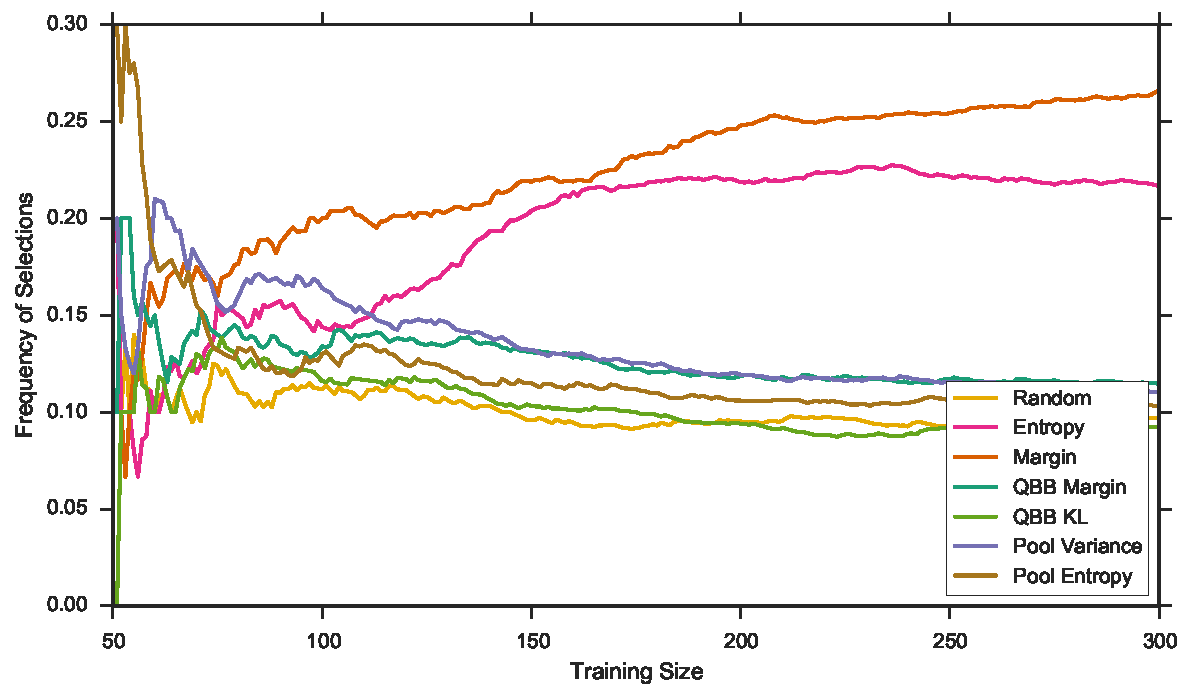
\includegraphics[width=\textwidth]{figures/5_thompson/vstatlas_ul_frequencies}
		\caption{Unbalanced pool and logistic regression}
		\label{fig:vstatlas_ul_frequencies}
	\end{subfigure}%
	\begin{subfigure}{.5\textwidth}
		\centering
		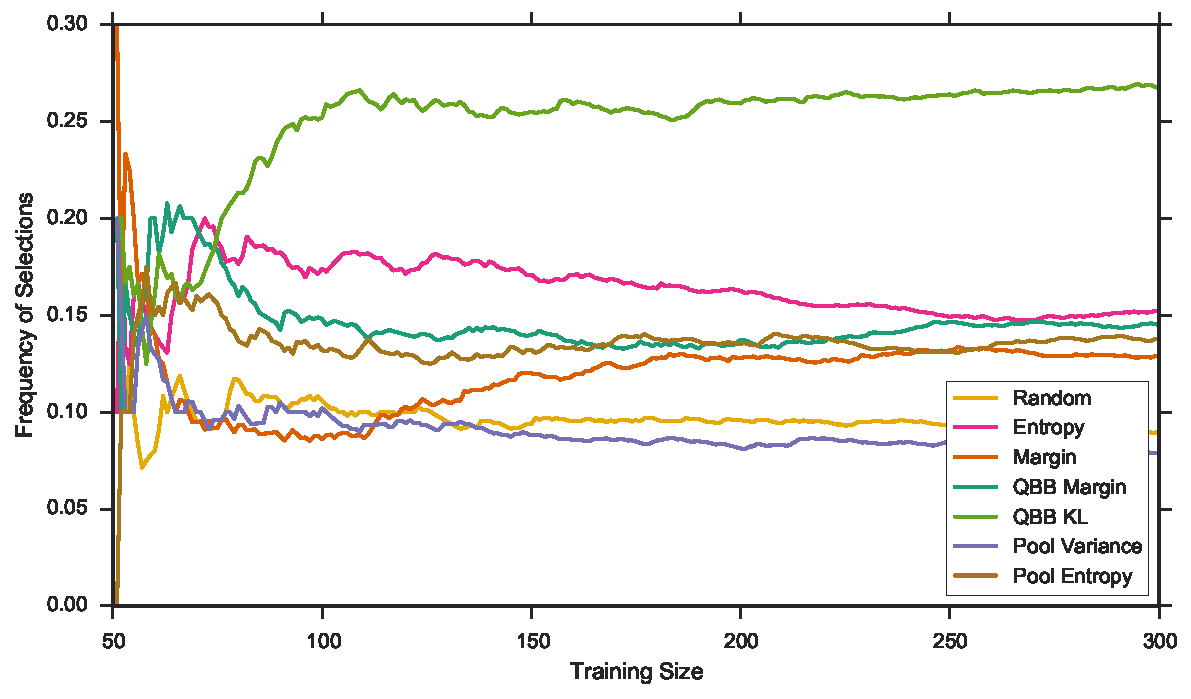
\includegraphics[width=\linewidth]{figures/5_thompson/vstatlas_ur_frequencies}
		\caption{Unbalanced pool and RBF SVM}
		\label{fig:vstatlas_ur_frequencies}
	\end{subfigure}
	\caption[Heuristic selection frequency (VST ATLAS)]{
		Heuristic selection frequency in Thopmson sampling with the VST ATLAS dataset.}
	\label{fig:vstatlas_frequencies}
\end{figure}


\begin{figure}[p]
	\centering
	\begin{subfigure}{.5\textwidth}
		\centering
		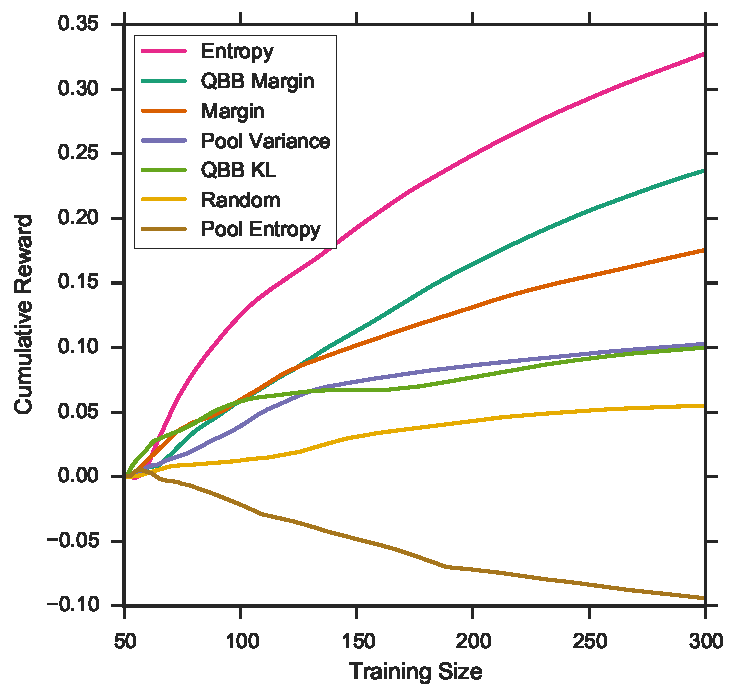
\includegraphics[width=\textwidth]{figures/5_thompson/vstatlas_bl_sum_rewards}
		\caption{Balanced pool and logistic regression}
		\label{fig:vstatlas_bl_sum_rewards}
	\end{subfigure}%
	\begin{subfigure}{.5\textwidth}
		\centering
		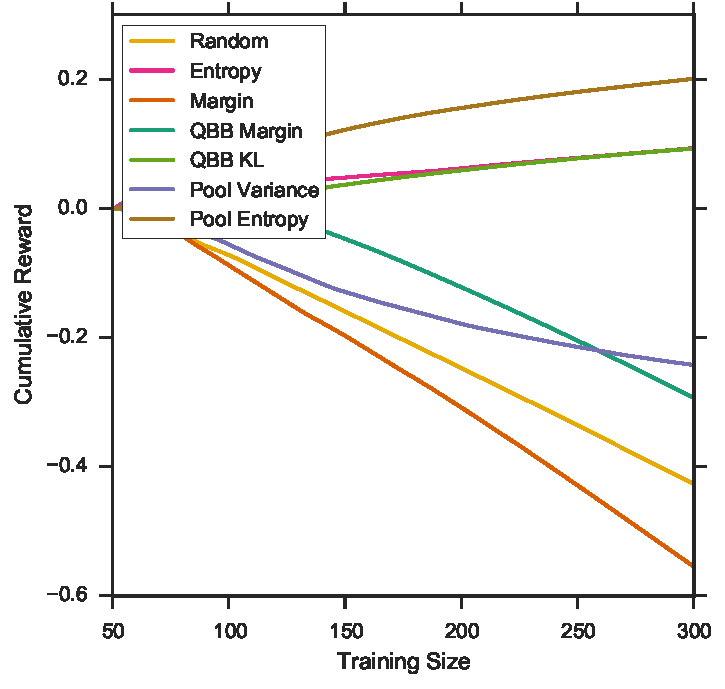
\includegraphics[width=\linewidth]{figures/5_thompson/vstatlas_br_sum_rewards}
		\caption{Balanced pool and RBF SVM}
		\label{fig:vstatlas_br_sum_rewards}
	\end{subfigure}
	\begin{subfigure}{.5\textwidth}
		\centering
		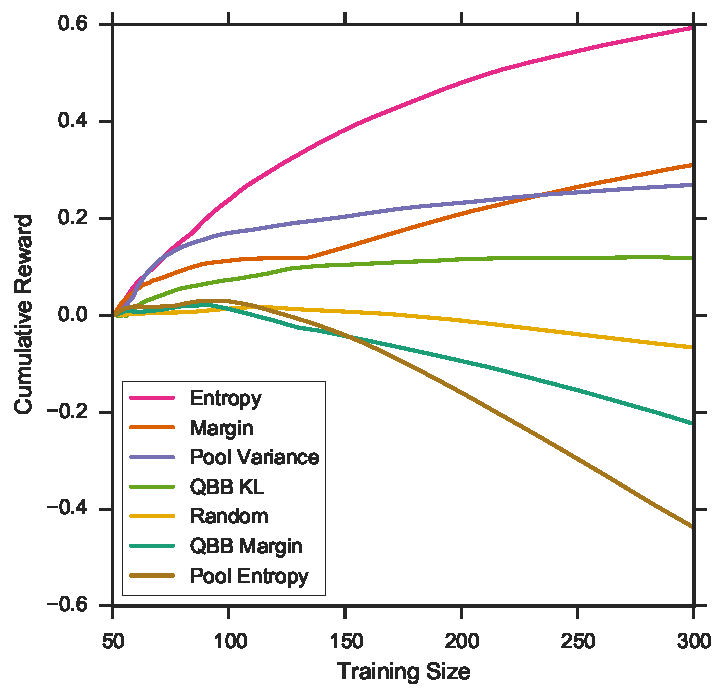
\includegraphics[width=\textwidth]{figures/5_thompson/vstatlas_ul_sum_rewards}
		\caption{Unbalanced pool and logistic regression}
		\label{fig:vstatlas_ul_sum_rewards}
	\end{subfigure}%
	\begin{subfigure}{.5\textwidth}
		\centering
		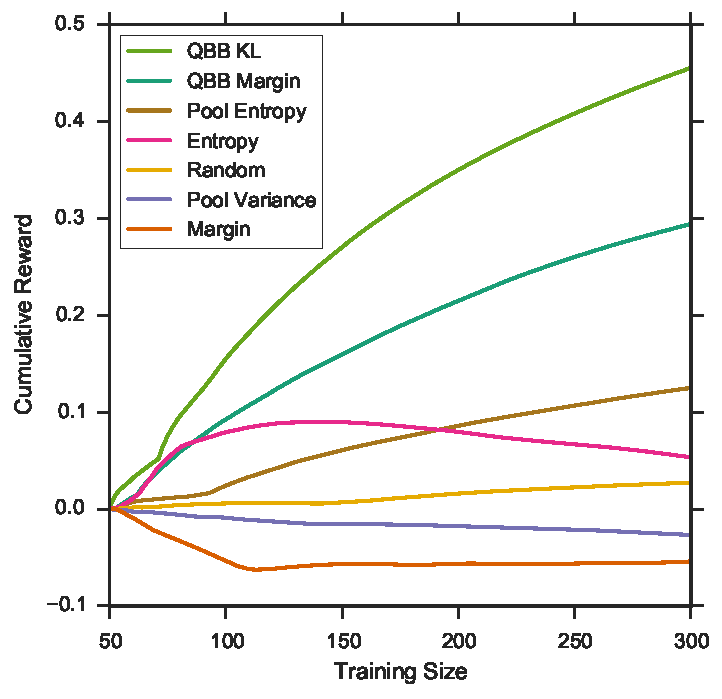
\includegraphics[width=\linewidth]{figures/5_thompson/vstatlas_ur_sum_rewards}
		\caption{Unbalanced pool and RBF SVM}
		\label{fig:vstatlas_ur_sum_rewards}
	\end{subfigure}
	\caption[Cumulative reward of heuristics (VST ATLAS)]{
		Cumulative reward in Thompson sampling with the VST ATLAS dataset.}
	\label{fig:vstatlas_sum_rewards}
\end{figure}


\begin{figure}[p]
	\centering
	\begin{subfigure}{.5\textwidth}
		\centering
		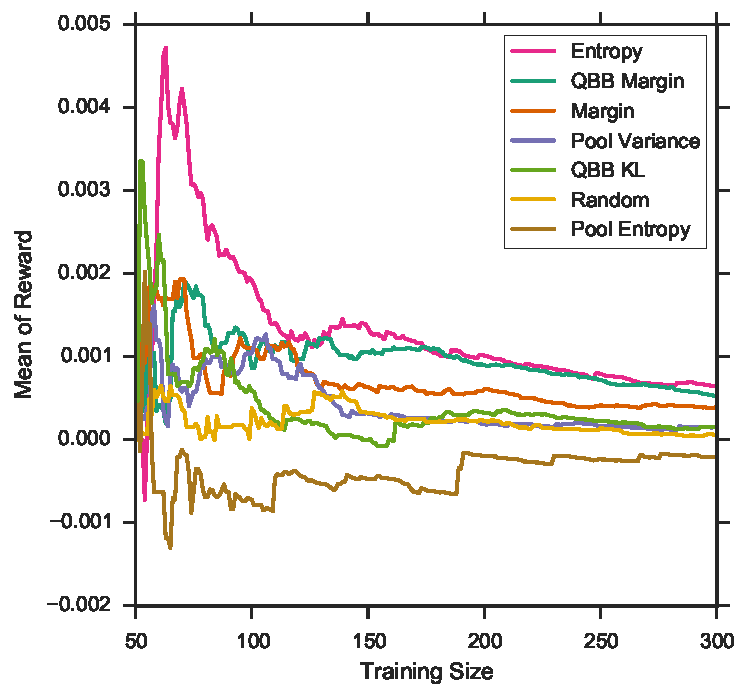
\includegraphics[width=\textwidth]{figures/5_thompson/vstatlas_bl_avg_rewards}
		\caption{Balanced pool and logistic regression}
		\label{fig:vstatlas_bl_avg_rewards}
	\end{subfigure}%
	\begin{subfigure}{.5\textwidth}
		\centering
		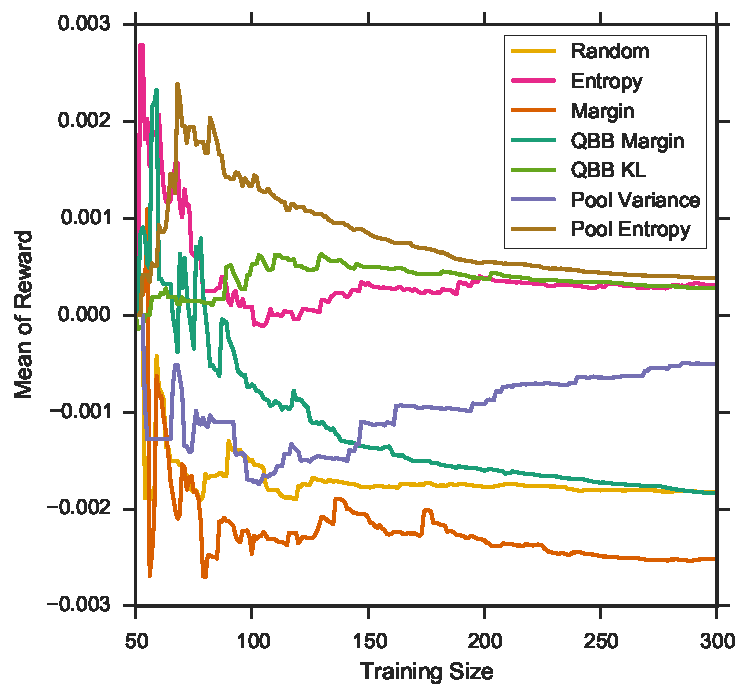
\includegraphics[width=\linewidth]{figures/5_thompson/vstatlas_br_avg_rewards}
		\caption{Balanced pool and RBF SVM}
		\label{fig:vstatlas_br_avg_rewards}
	\end{subfigure}
	\begin{subfigure}{.5\textwidth}
		\centering
		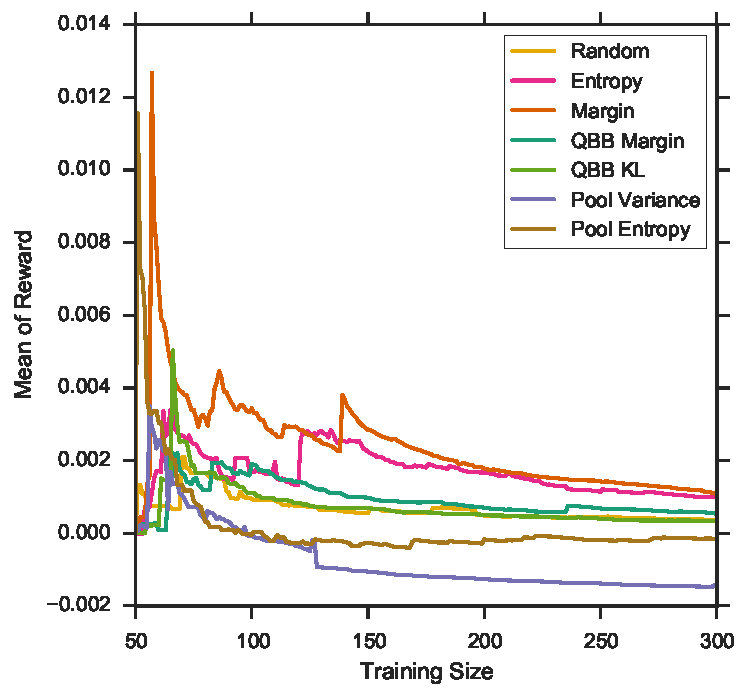
\includegraphics[width=\textwidth]{figures/5_thompson/vstatlas_ul_avg_rewards}
		\caption{Unbalanced pool and logistic regression}
		\label{fig:vstatlas_ul_avg_rewards}
	\end{subfigure}%
	\begin{subfigure}{.5\textwidth}
		\centering
		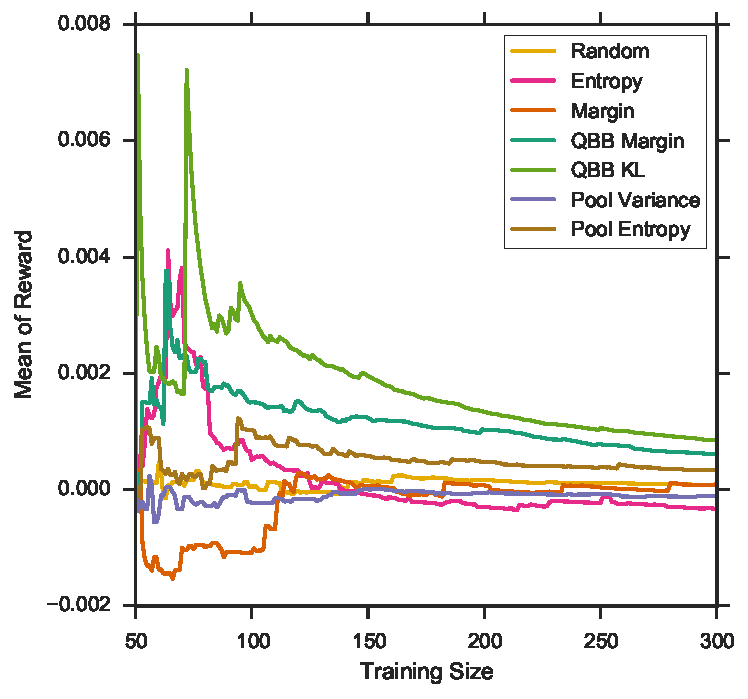
\includegraphics[width=\linewidth]{figures/5_thompson/vstatlas_ur_avg_rewards}
		\caption{Unbalanced pool and RBF SVM}
		\label{fig:vstatlas_ur_avg_rewards}
	\end{subfigure}
	\caption[Mean reward of heuristics (VST ATLAS)]{
		Mean reward in Thompson sampling with the VST ATLAS dataset.}
	\label{fig:vstatlas_avg_rewards}
\end{figure}
%%% Local Variables: 
%%% mode: latex
%%% TeX-master: "thesis"
%%% End: 
